\documentclass[oneside,a4paper]{article}

% ========== Preamble (packages, definitions etc.) ==========

\usepackage[utf8]{inputenc}
\usepackage[english]{babel}
\usepackage{graphicx}
\usepackage{xcolor}
\usepackage{amsmath, amsthm, amssymb}
\usepackage{csquotes}
\usepackage{hyperref}
\usepackage{listings}
\usepackage{lmodern}
\usepackage{color}
\usepackage{listings}
\lstset{
    breaklines=true,
    basicstyle=\tt\normalsize,
    keywordstyle=\color{blue},
    identifierstyle=\color{magenta},
    frame = single
} 
%\usepackage[backend=bibtex,style=abbrv]{biblatex}
\newcommand{\todo}[1]{{\color{blue}#1}}  % show to-do items in blue
\setlength{\parskip}{\baselineskip}
\usepackage[activate={true,nocompatibility},
            final,
            tracking=true,
            kerning=true,
            %spacing=nonfrench,
            factor=1100,
            stretch=10,
            shrink=10,
            nopatch=eqnum]{microtype}
%\hypersetup{
%    pdftitle={},
%    bookmarks=true,
%    pdfpagemode=FullScreen,
%}

\newcounter{questionnum} \setcounter{questionnum}{0}
%\newcommand{\question}[1]{%
%  \refstepcounter{questionnum}%
%  \paragraph{Question~\arabic{questionnum}:}{\emph{#1}}}

\newcommand\filltoend{\leavevmode{\unskip
  \leaders\hrule height.5ex depth\dimexpr-.5ex+0.4pt\hfill\hbox{}%
  \parfillskip=0pt\endgraf}}

\newcommand{\problem}[2]{%
	\vspace{-0.7em}
	\hspace{0.02\textwidth}
	\begin{minipage}[t][][b]{0.95\textwidth}
		{\bf \hspace{-0.015\textwidth}\makebox[7.5em][l]{{#1} ~~\filltoend}}%
		\hspace{1.2mm}{\it #2}%
	\end{minipage}
}

\def\email#1{{\tt#1}}

\lstset{ % Set the default style for code listings
	numbers=left,
	numberstyle=\scriptsize,
	numbersep=8pt,
	basicstyle=\scriptsize\ttfamily,
	keywordstyle=\color{blue},
	stringstyle=\color{red},
	commentstyle=\color{green!70!black},
	breaklines=true,
	frame=single,
	language=bash,
	tabsize=4,
	showstringspaces=false
}
\usepackage{svg}
\usepackage{float}
\usepackage[margin=2cm]{geometry}
\usepackage{pdfpages}
\usepackage[title]{appendix}
\usepackage{indentfirst}
\usepackage{caption, subcaption}
\usepackage{enumitem}


% ========== Title page ==========

\title{
	
\includegraphics[width=0.6\textwidth]{UU_logo.pdf}\\[1em]
	Computer-Assisted Image Analysis I - 1TD396\\[1em]
	Computer Exercise 1\\[3em]
}

\author{
	Jyong-Jhih Lin, \and Linus Falk, \and Niklas Kostrzewa, \and Teng-Sung Yu
	%
}

\date{November 03, 2022}

\begin{document}

\maketitle
\thispagestyle{empty} % Removes page number for front page
\pagebreak

% ========== Document contents ==========
\section*{Q1}
\textbf{Where in the image is the pixel (1,1) located and what is the graylevel value? In command window type I(1,1). Did you get the same value?}

Upper left corner value: 89
\begin{lstlisting}[language=MATLAB]
imtool(I);
I(1,1); 
Return: uint8 89
\end{lstlisting}


\section*{Q2}
\textbf{Explain what contrast and brightness are and include figures of the histograms of the images napoleon.png, napoleon light.png, and napoleon dark.png. Can you tell from the histograms which figure has the highest contrast and which figure is the brightest?}

A image with high contrast will have a broader distribution of values often with peaks widely separated. While a low contrast picture will be narrower distributed. The brighter image will have its histogram further to the higher numbers in the histogram.

'napoleon.png' has the highest contrast.
'napoleon light.png' is the brightest.

\begin{lstlisting}[language=MATLAB]
listofim = ["napoleon.png", "napoleon_light.png", "napoleon_dark.png"];

I1 = imread(listofim(1));
I2 = imread(listofim(2));
I3 = imread(listofim(3));


bins = 256;
hold on;

subplot(3,1,1);
histogram(single(I1(:)),bins)
title('High contrast: ' + listofim(1))
xlim([0 256])

subplot(3,1,2)
histogram(single(I2(:)),bins)
xlim([0 256])
title('Brighter: ' + listofim(2))

subplot(3,1,3)
histogram(single(I3(:)),bins)
xlim([0 256])
title('Darker: ' + listofim(3))
\end{lstlisting}




\section*{Q3}
\textbf{Explain the difference of imagesc((I/64)*64) and imagesc((Is/64)*64), where I is uint8
and Is is single.}

uint8 is an integer datatype, and its value is between 0 ~ 256. If you divided it by 64, there will be only 5 possible value (0~4) for each pixel. Therefore, after multiple by 64, there are still only five kind of values, so it will result in a vague image. Single is a float datatype, when it divided by 64, you retain all unique numbers, since the precision is a lot higher.
\newline
\newline
\newline
\begin{figure}[ht!]
\centering
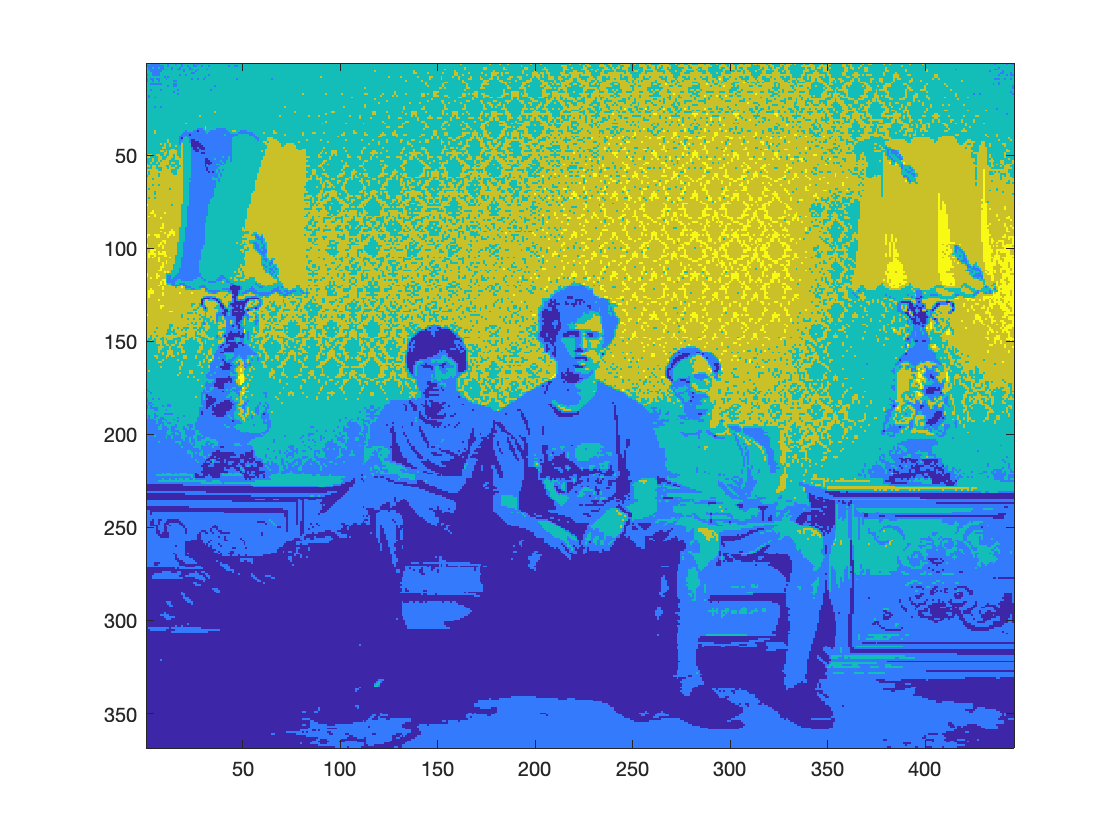
\includegraphics[width=100mm]{figures/Q3_img_uint8.png}
\caption{image of uint8 datatype}
\label{fig:Q3a}
\end{figure}

\begin{figure}[ht!]
\centering
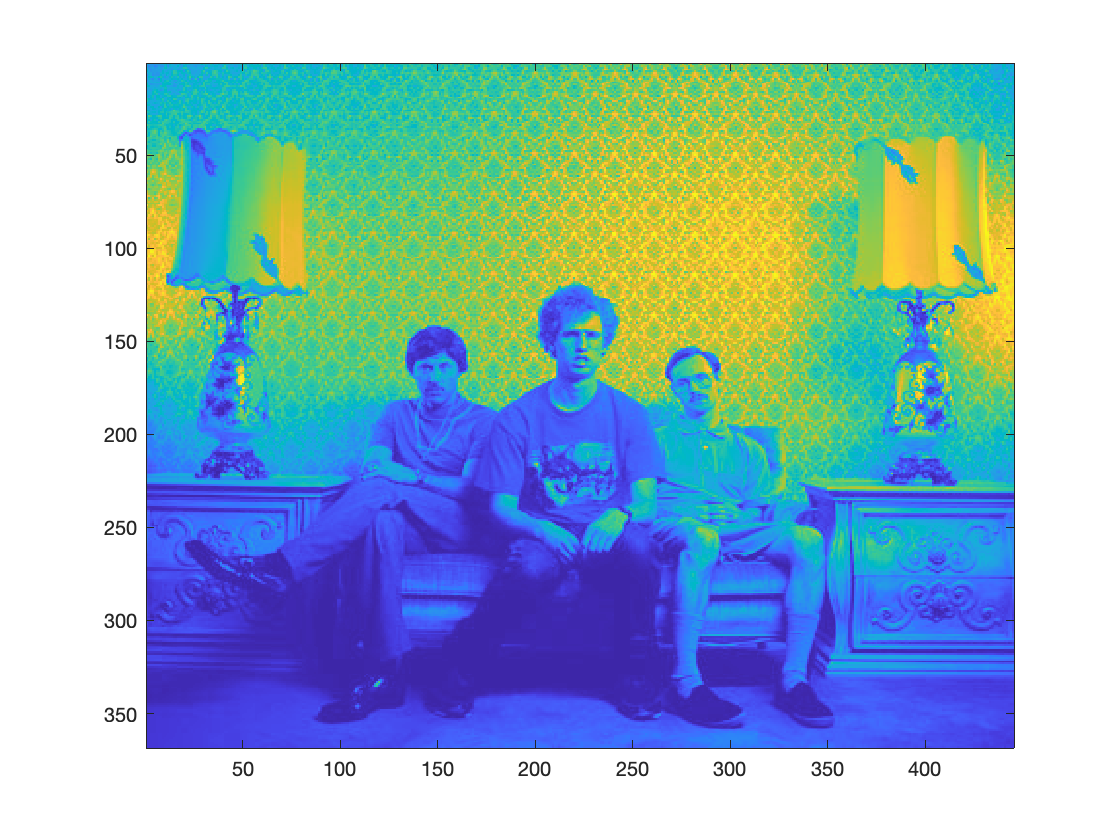
\includegraphics[width=100mm]{figures/Q3_img_single.png}
\caption{image of single datatype}
\label{fig:Q3b}
\end{figure}



\section*{Q4}
\textbf{Demonstrate a mathematical expression involving I to make it brighter.}

Q4 we add a constant g(x,y) =f(x,y) + C, where C is a positive value.

\begin{lstlisting}[language=MATLAB]
%Q4
subplot(2,1,1)
imshow(I + 100)
title('I+100')

%Q5
subplot(2,1,2)
imshow(I * 0.5)
title('I * 0.5')
\end{lstlisting}

\section*{Q5}
\textbf{Demonstrate a mathematical expression involving I to give it lower contrast.}

Q5 lower contrast multiply with  0 $<$ C $<1$,  g(x,y) = f(x,y) $\times$ C.


\section{Q6}
\textbf{Use g = 2 and g = 12 and explain the resulting images.}

Gamma function(2) generates a overall darker image. By raise the image to the power of chosen gamma/lambda and then normalizing it to the correct range. We can see the cumulative histogram start of with a steep slope at the start indicating that the number of pixels with low value is higher then with low. 

Gammafunction(0.5) generates an overall brighter image were the steep part of the image is pushed further to the higher values, right side of the cumulative histogram. 


\begin{figure}[ht!]
\centering
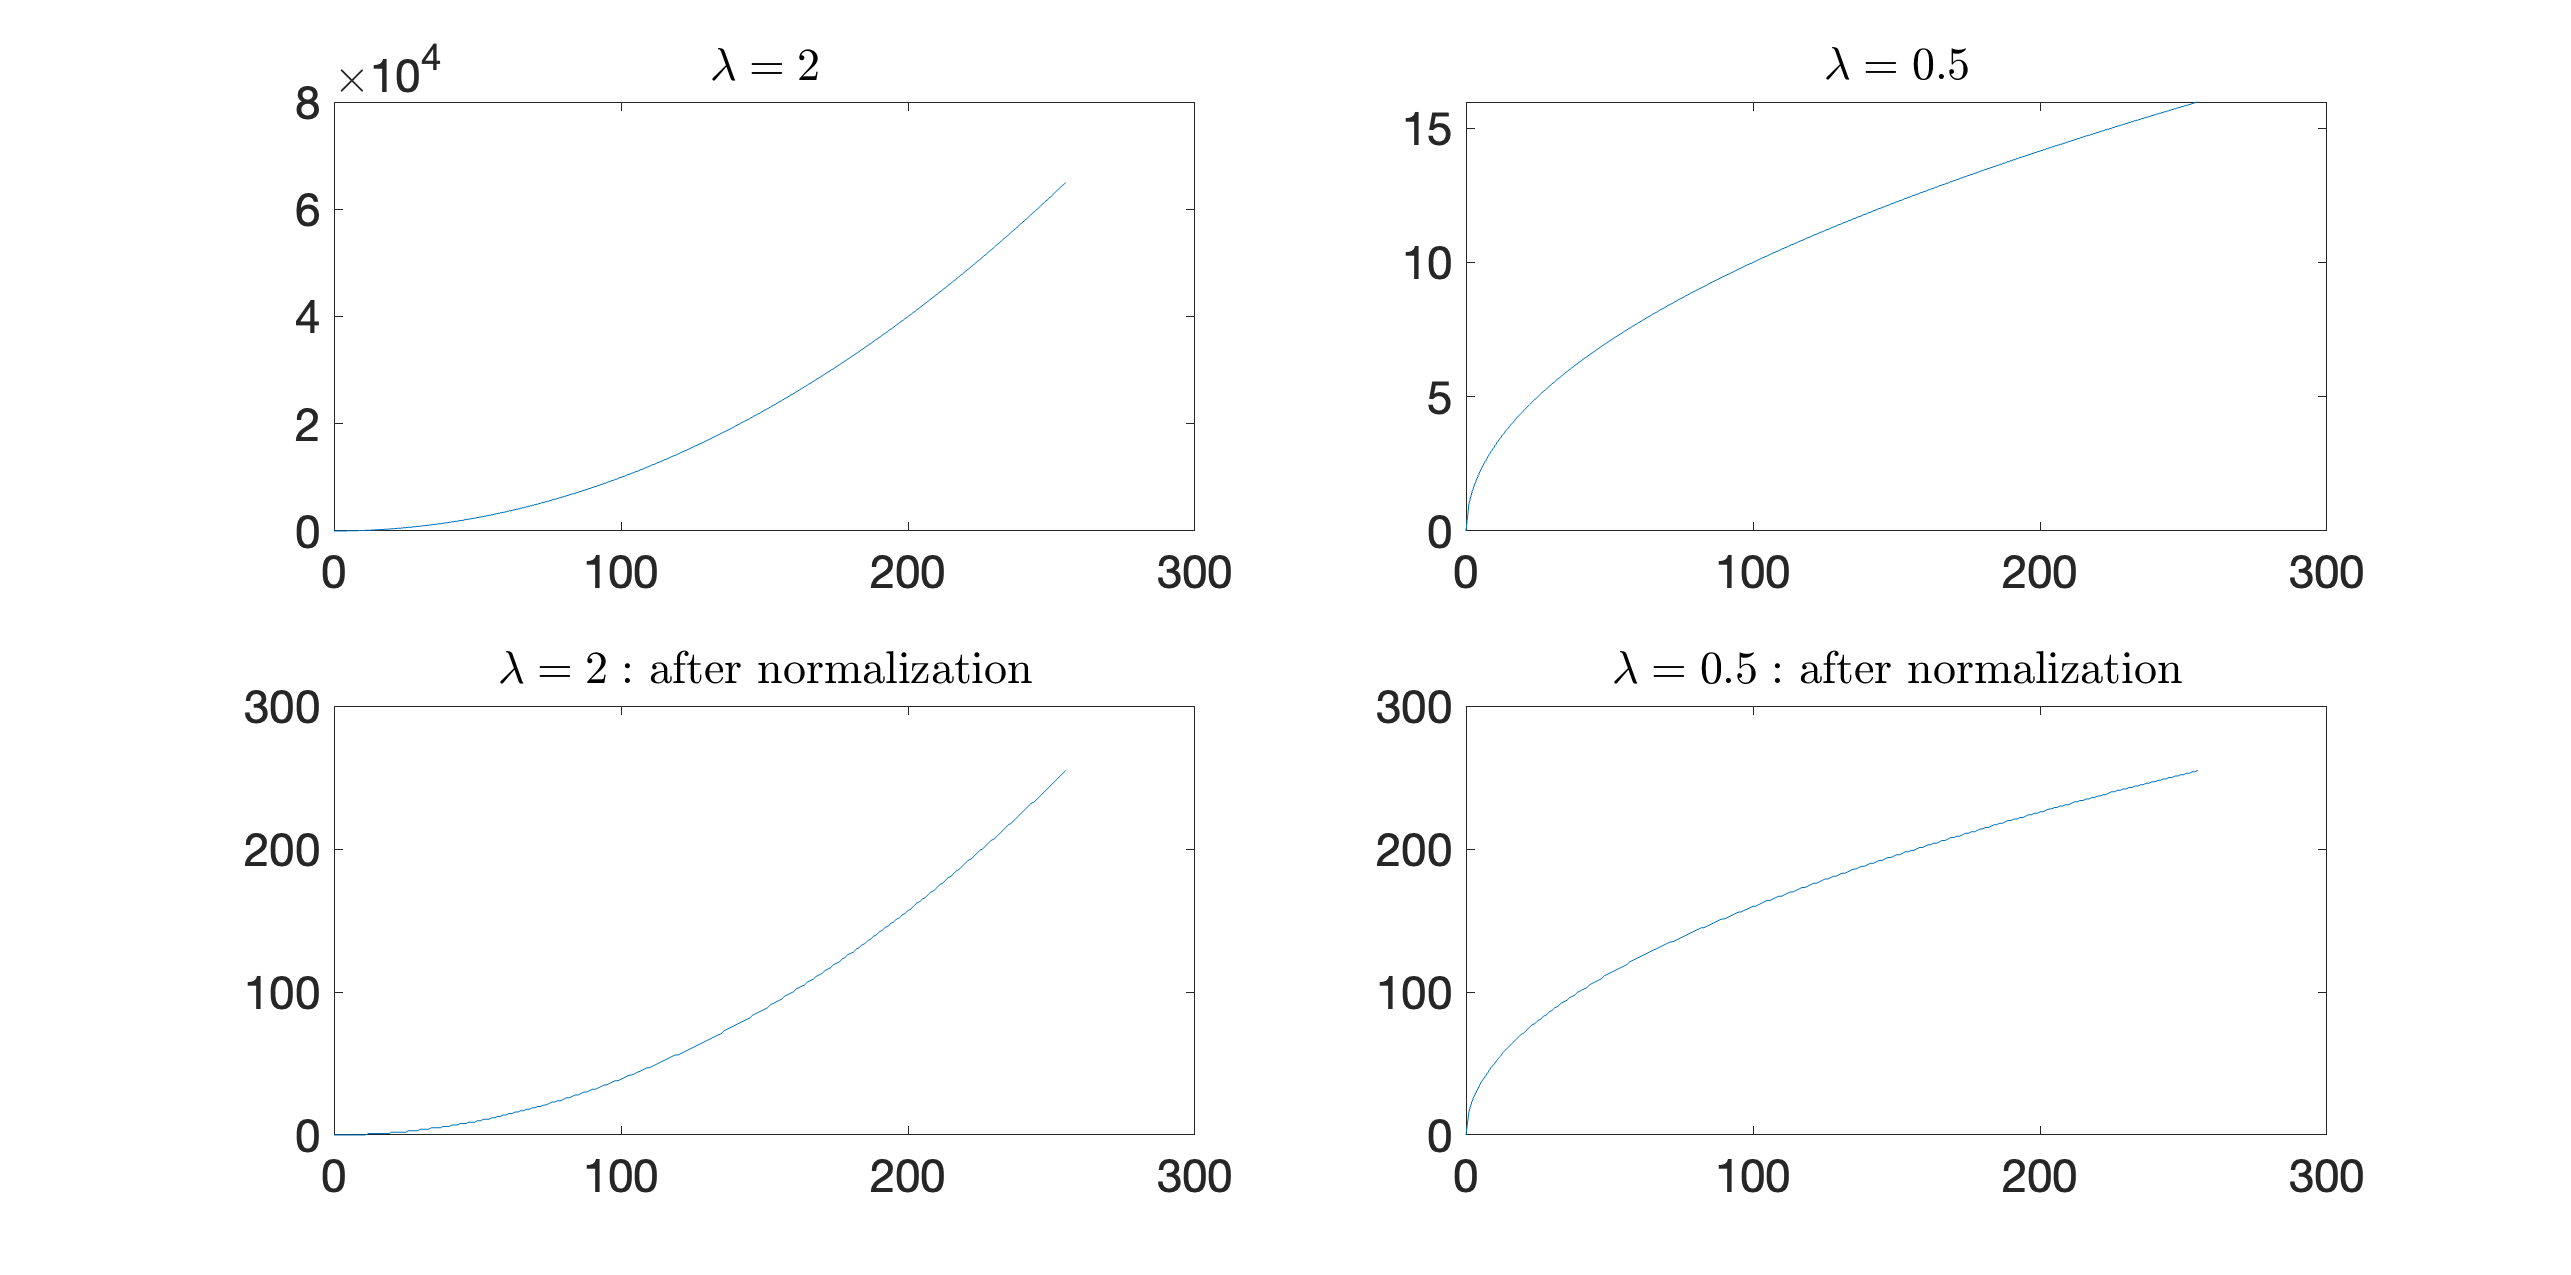
\includegraphics[width=100mm]{figures/Q6b.png}
\caption{Example of caption}
\label{fig:Q6b}
\end{figure}

\begin{figure}[ht!]
\centering
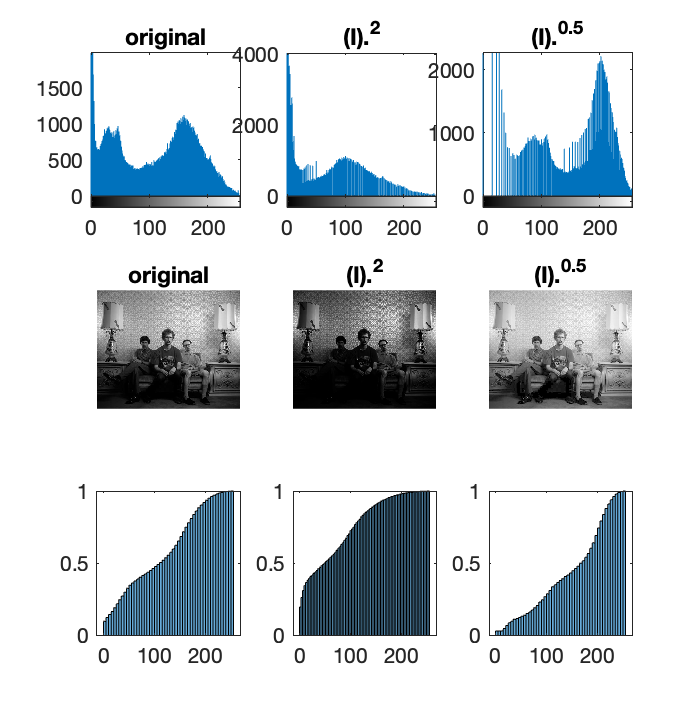
\includegraphics[width=100mm]{figures/Q6.png}
\caption{Example of caption}
\label{fig:Q6}
\end{figure}

\begin{lstlisting}[language=MATLAB]
listofim = ["napoleon.png", "napoleon_light.png", "napoleon_dark.png"];

I = imread(listofim(1));

L = double(I).^2;
out1 = uint8(L .* (255/max(max(L)))); 
L = double(I).^0.5;
out2 = uint8(L .* (255/max(max(L)))); 

figure(3);
I = imread('napoleon.png'); 
subplot(3,3,1)
imhist(I);
title('original')
subplot(3,3,2)
imhist(out1);
title('(I).^2')
subplot(3,3,3)
imhist(out2);
title('(I).^{0.5}')
subplot(3,3,4)
imshow(I)
title('original')
subplot(3,3,5)
imshow(out1)
title('(I).^2')
subplot(3,3,6)
imshow(out2)
title('(I).^{0.5}')
subplot(3,3,7)
histogram(I,'Normalization','cdf');
subplot(3,3,8)
histogram(out1,'Normalization','cdf');
subplot(3,3,9)
histogram(out2,'Normalization','cdf');
\end{lstlisting}


\section*{Q7}
\textbf{Explain how histogram equalization works in theory. Include histograms of one of the images before and after applying equalization in your report and explain what you see. Do the changes to the histograms and the images agree with the theory of histogram equalization?}

Histogram equalization is a way to distribute the intensity values in a more uniform way in an image by busing the cumulative density function . Perfectly evenly distributed intensities is represented by a straight line in the cumulative distribution. 

\begin{figure}[ht!]
\centering
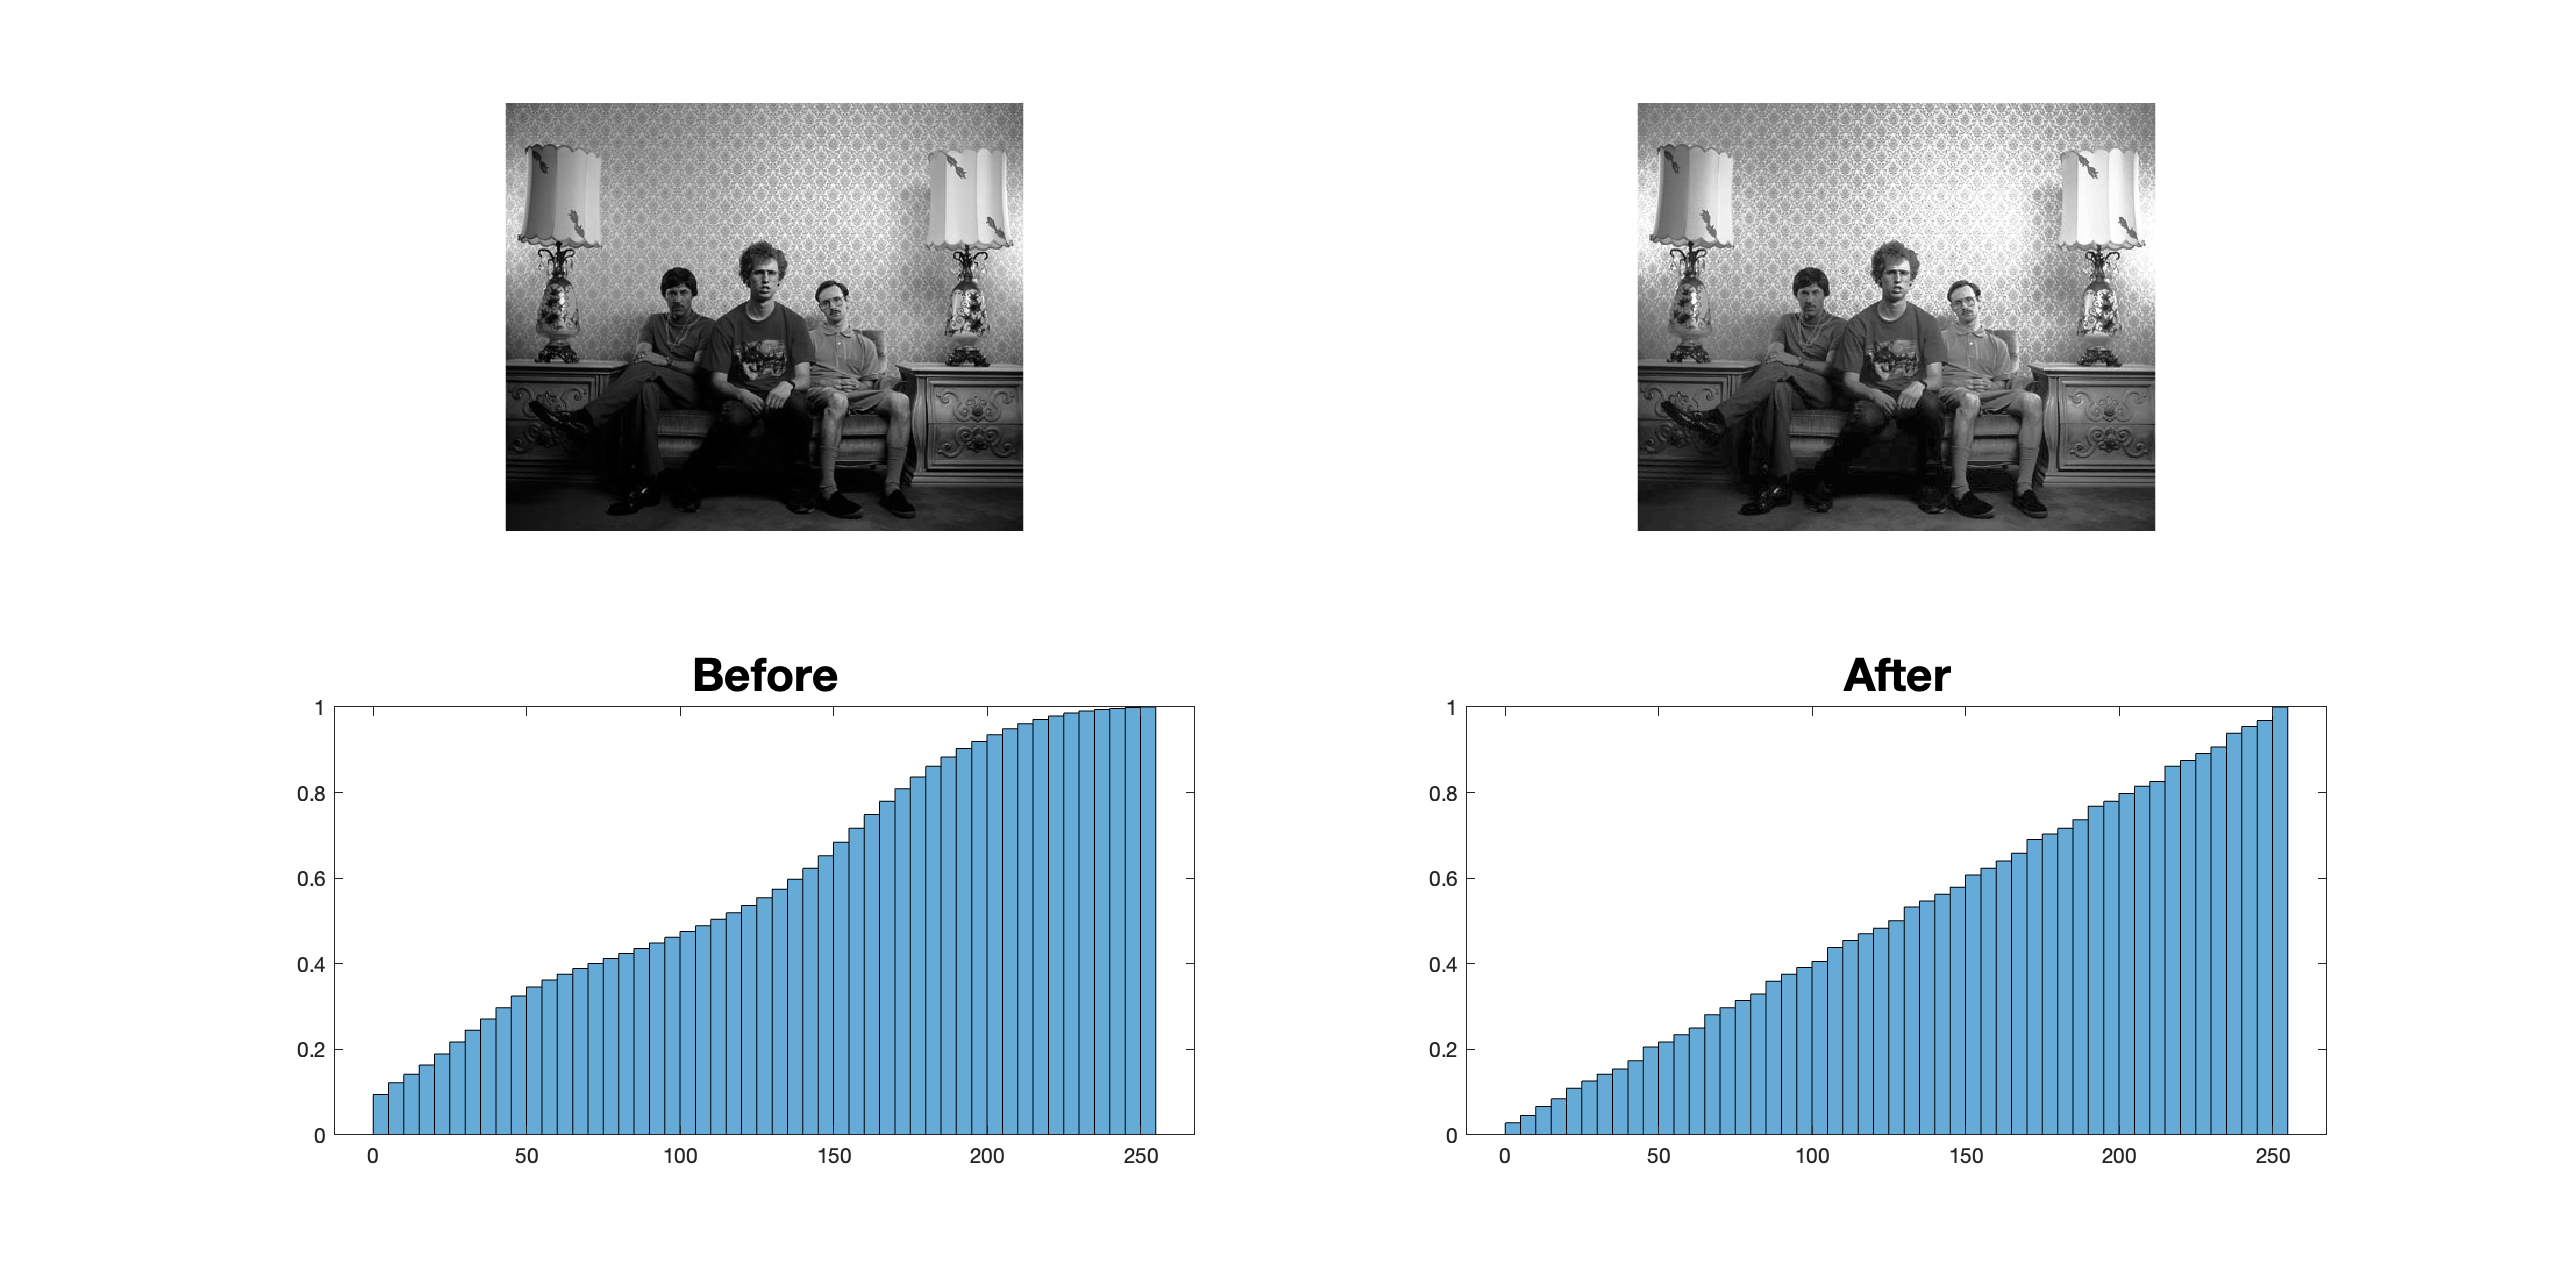
\includegraphics[width=120mm]{figures/Q11b.png}
\caption{}
\label{fig:Q11b}
\end{figure}


\section*{Q8}
\textbf{Explain the role of the interpolation method as well as the role of the lowpass-filter. Which combination of options do you prefer? And why?}
Interpolation is used when resizing the image to make it larger or fill in gaps when a image is rotated. The new pixels must be assigned values and this is done using interpolation methods: nearest or bilinear. Nearest means that we assign the new pixel the value of the nearest point it falls within, (better explained with \ref{fig:bilinear})
Bilinear interpolation uses the weighted average of the nearest $2 \times 2$ pixels.   

\textcolor{red}{Add example picture from lab?}

\begin{figure}[ht!]
\centering
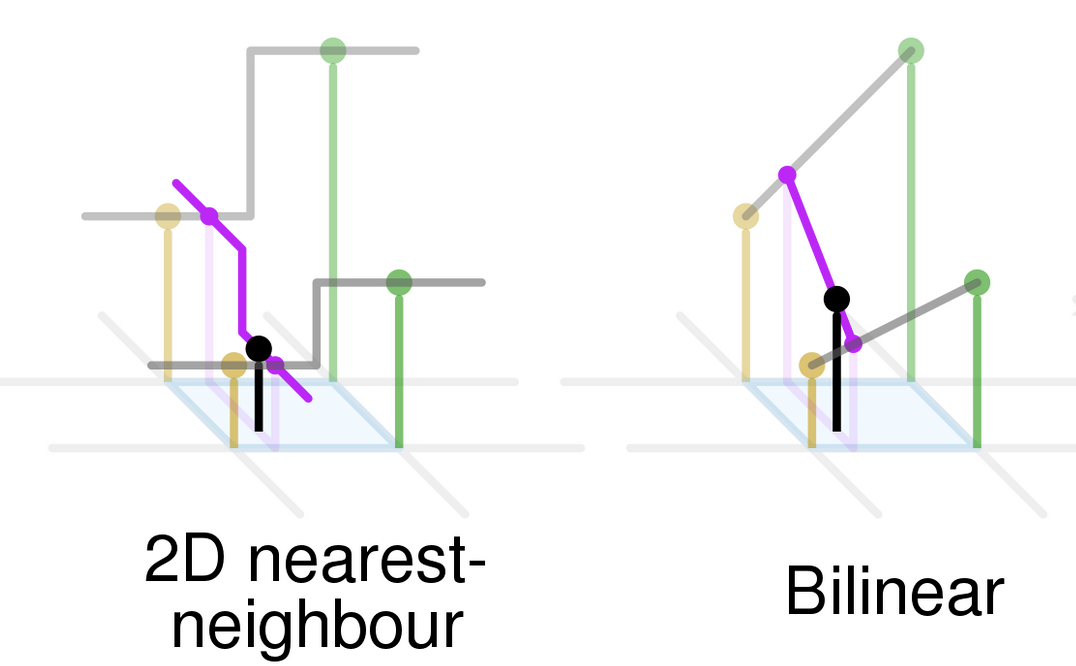
\includegraphics[width=80mm]{figures/Nearest_bilinear.png}
\caption{\url{https://en.wikipedia.org/wiki/Nearest-neighbor_interpolation\#/media/File:Comparison_of_1D_and_2D_interpolation.svg}}
\label{fig:bilinear}
\end{figure}

\textcolor{red}{fix reference}

Anti aliasing filter or lowpass filter is used to remove higher frequency content of the image to avoid that this information corrupts the output image after under sampling it. 


\section*{Q9}
\textbf{Can you give a real-life example of aliasing outside the area of image analysis and signal processing in general? Have you seen this phenomenon before?}

Striped sweater while having a video/conference call. 

\section*{Q10}
\textbf{How can a “standard” healthy brain, or a mean image, of the two images brain1.png and brain2.png be constructed? In your report include a figure showing the standard brain.}
The mean can be created by adding the images together pixel wise and divide by the total number of images. In this case we add two images together and therefore divide by 2. One must be careful with the addition because of the data type the image is stored in. Addition easily results in "overflow". Therefore dividing by the number of images and then add them.  


\begin{lstlisting}[language=MATLAB]
Brain1 = imread('brain1.png');
Brain2 = imread('brain2.png');
Brain3 = imread('brain3.png');

standard_brain = imadd(single(Brain1), single(Brain2));
standard_brain = standard_brain./2;
figure
imshow(uint8(standard_brain))
\end{lstlisting}

\begin{figure}[ht!]
\centering
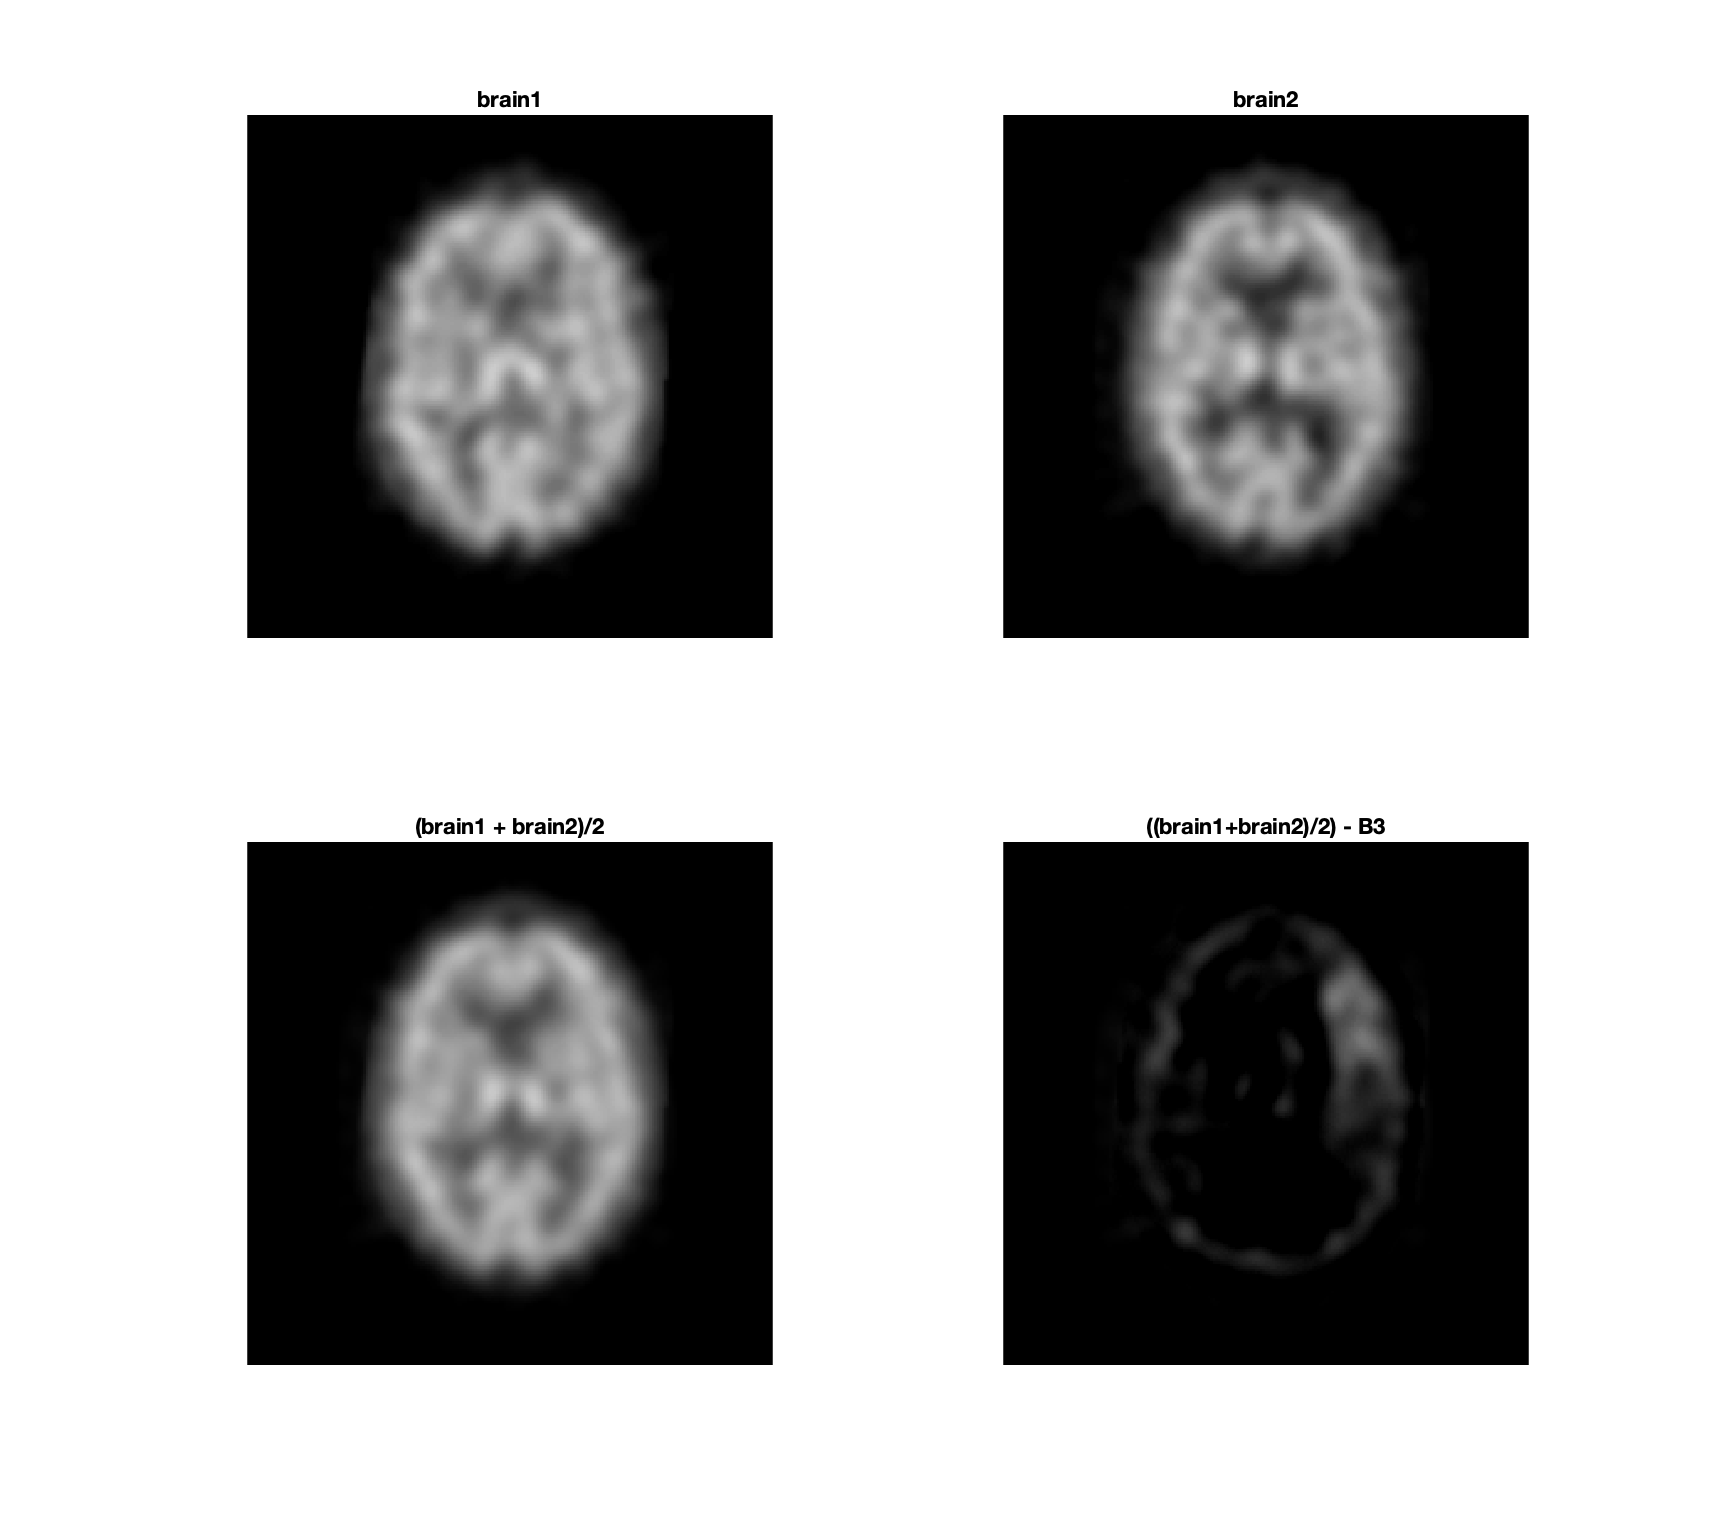
\includegraphics[width=100mm]{figures/Q11.png}
\caption{standard brain upper left}
\label{fig:Q10}
\end{figure}

\section{Q11}
\textbf{Find the difference between the “standard” brain and the image from the stroke patient
(brain3.png). Where in the brain is the change located?}

Upper right corner of the image? Right frontal lobe




\section*{Q12}
\textbf{What happens when a pixel gets a value less than 0 or a value greater than 255? Are there other ways this can be handled? Did you think of this when you computed the “standard” brain in the previous exercise?}

It becomes/stay zero if you subtract such that it would become negative, the same applies the other way: stay 255 if you add more to it. LF: Did not consider this in the first try but became aware of it when plotting the added brain images without division "burned out highlights". 


\section*{Q13}
\textbf{Compare rotations performed with and without interpolation. It is easiest to see differences along lines and edges of the images. What does interpolation mean in this case?}

When rotating a image the repositioning of the pixels makes it necessary to take some sort of average when a pixel ends up on a boarder between pixels. 

\begin{figure}[ht!]
\centering
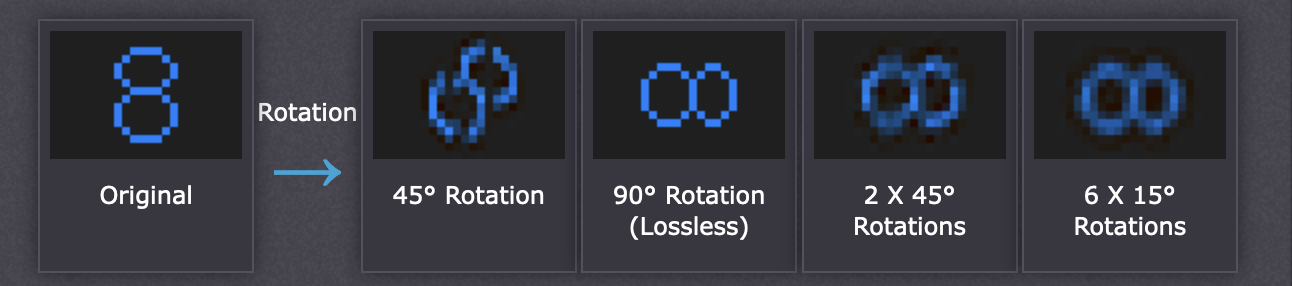
\includegraphics[width=120mm]{figures/Screenshot 2022-11-03 at 19.35.40.png}
\caption{source \url{https://www.cambridgeincolour.com/tutorials/image-interpolation.htm}}
\label{fig:example}
\end{figure}

\section*{Q14}
\textbf{In general it is faster to rotate the image by a multiple of 90 degrees than by some arbitrary degree. Explain why. For this task use Matlab functions tic and toc.}

It is faster because no pixel end up on a border between pixels and no mean is calculated, no interpolation. 

\begin{lstlisting}[language=MATLAB]
tic; 
for i=1:1000
    J = imrotate(I,20);
end
result_20deg = toc
tic;
for i=1:1000
    J = imrotate(I,90);
end
result_90deg = toc

Output:
result_20deg =
    0.2485

result_90deg =
    0.0833
\end{lstlisting}


\section*{Q15}

\begin{lstlisting}[language=MATLAB]
I = imread("my_image.jpg");

imshow(I)

J = rgb2gray(I);

subplot(1,2,1)
imshow(I)
title('Original')
subplot(1,2,2)
imshow(J)
title('rgb2gray')

targetSize = [683 683];

r = centerCropWindow2d(size(J),targetSize);
Jr = imcrop(J,r);
Jr = imresize(Jr, [128 128], 'bilinear', 'antialiasing', true);

figure(2)
imshow(Jr)


result = Jr;

padda = padarray(Jr,[2 2],0); 
result = padda;

for i=3:128
    for j = 3:128
        result(i,j) = mean(padda((i-2):(i+2),(j-2):(j+2)),'all');   
    end
end

result = padda(3:130, 3:130);
figure(3)
imshow(uint8(result))
1
subplot(1,3,1)
imshow(Jr)
title('Original', 'fontsize',22)
subplot(1,3,2)
imshow(result)
title('Filtered', 'fontsize',22)
subplot(1,3,3)
imshow(Jr-result)
title('Subtracted', 'fontsize',22)
print(gcf, '-dpng', 'Q15.png')
\end{lstlisting}

\begin{figure}[ht!]
\centering
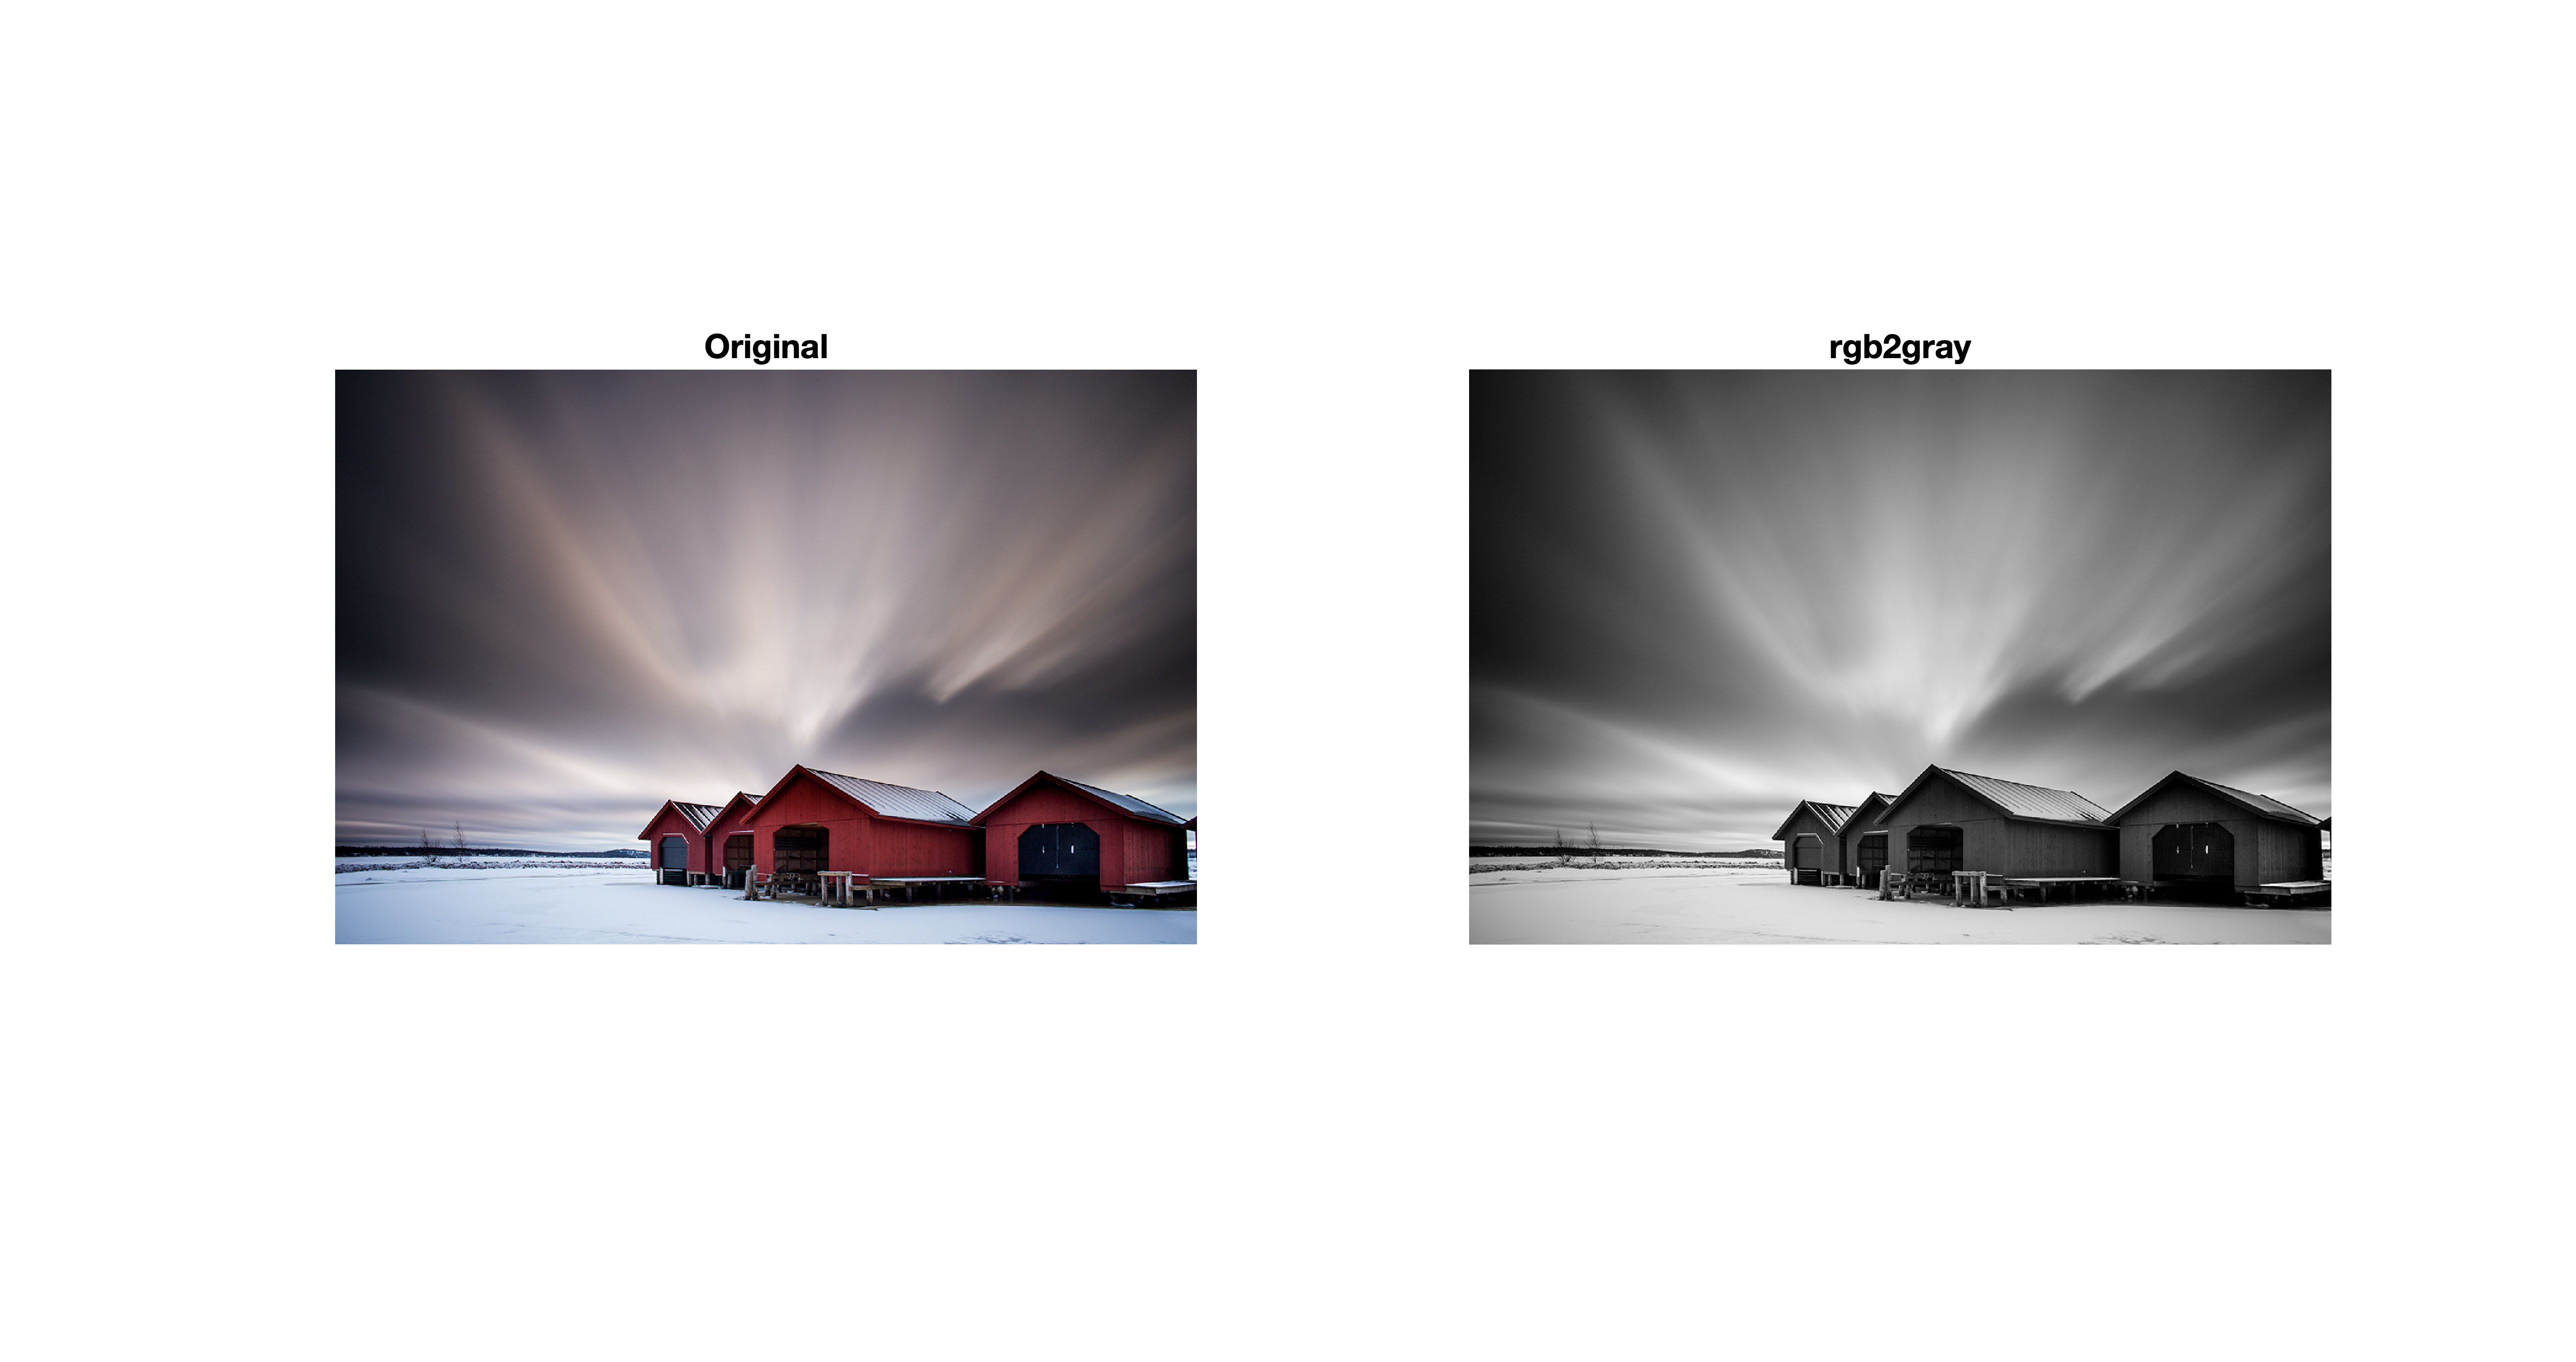
\includegraphics[width=140mm]{figures/Q15a.png}
\caption{Photo: Linus Falk}
\label{fig:Q15a}
\end{figure}

\begin{figure}[ht!]
\centering
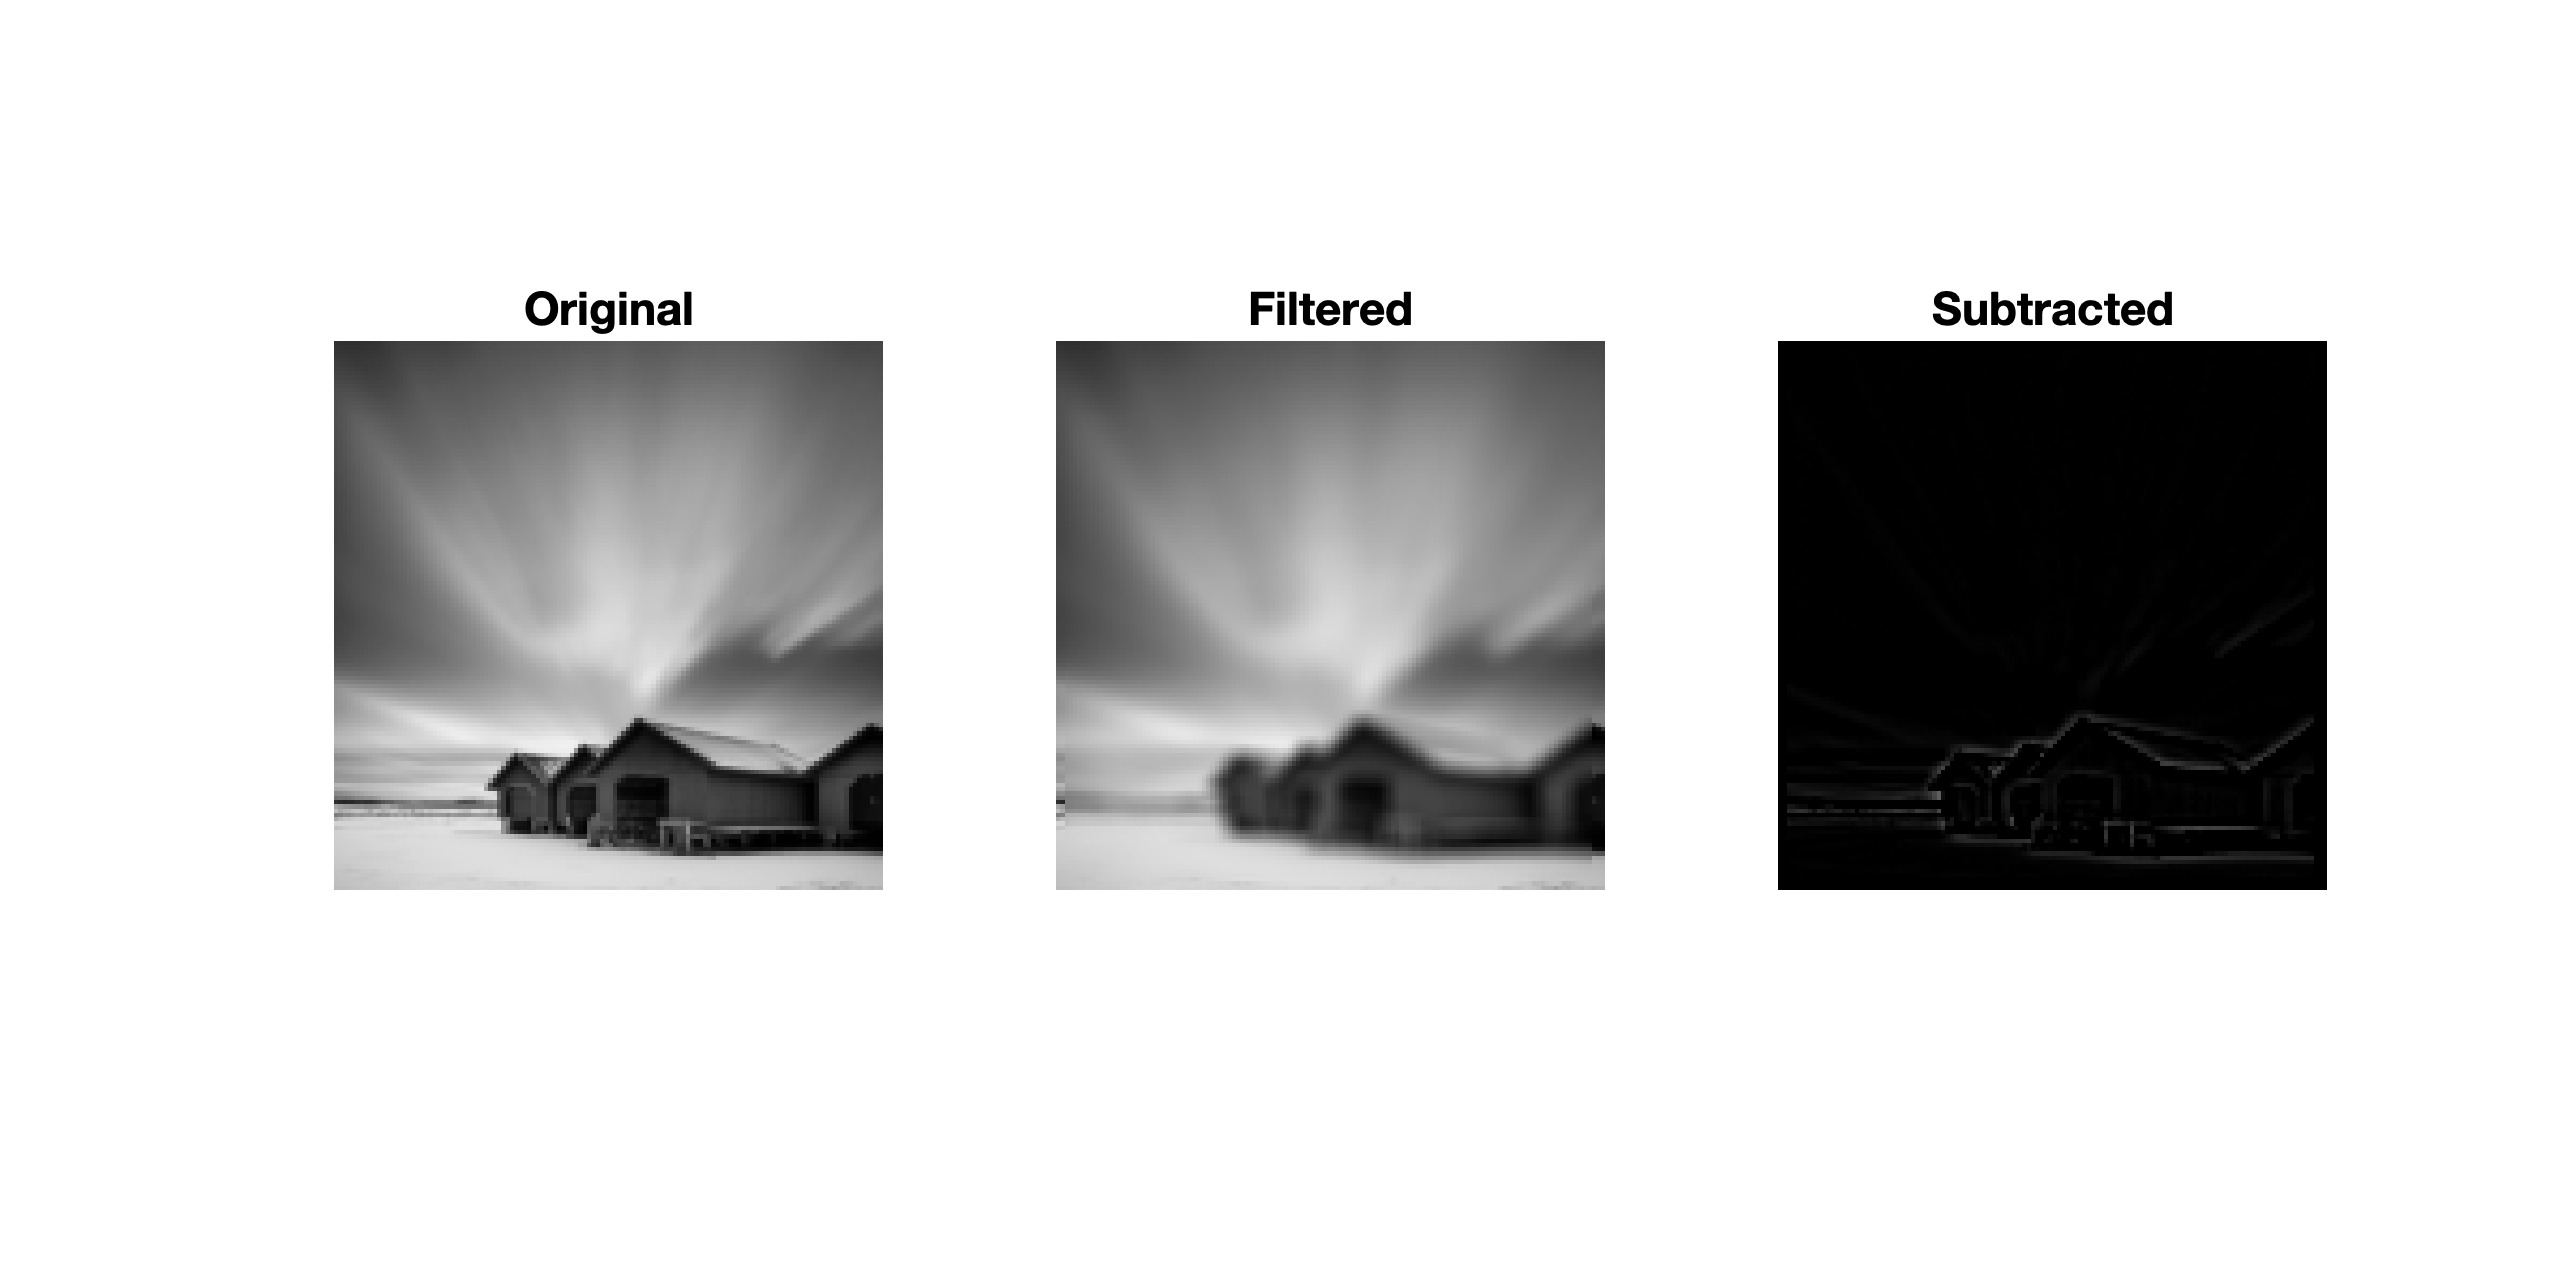
\includegraphics[width=140mm]{figures/Q15.png}
\caption{}
\label{fig:Q15}
\end{figure}

\section{Q16}
\begin{lstlisting}[language=MATLAB]
InI = Jr; %Input image
numofpixels=size(InI,1)*size(InI,2);
OutI = uint8(zeros(size(InI,1),size(InI,2))); %Output image
freq = zeros(256,1);
prob = zeros(256,1);

% Calculate frequency of pixel values and the 
% "probality of that pixel value"


for i=1:size(InI,1)
    for j=1:size(InI,2)
        val=InI(i,j);
        freq(val+1)=freq(val+1)+1;
        prob(val+1)=freq(val+1)/numofpixels;
    end
end

% Calculate the transformation by calculating the cdf 
% 
sum=0;
no_bins=255;
cum = cumsum(freq);
probcum = cum./numofpixels;
output = round(probcum.*no_bins);


for i=1:size(InI,1)
    for j=1:size(InI,2)
            OutI(i,j)=output(InI(i,j)+1);
    end
end

subplot(3,1,1)
imshow(OutI);
subplot(3,1,2)
histogram(OutI);
subplot(3,1,3)
histogram(OutI,'Normalization','cdf');
title('Histogram equalization');
print(gcf, '-dpng', 'Q16.png')
\end{lstlisting}

\begin{figure}[ht!]
\centering
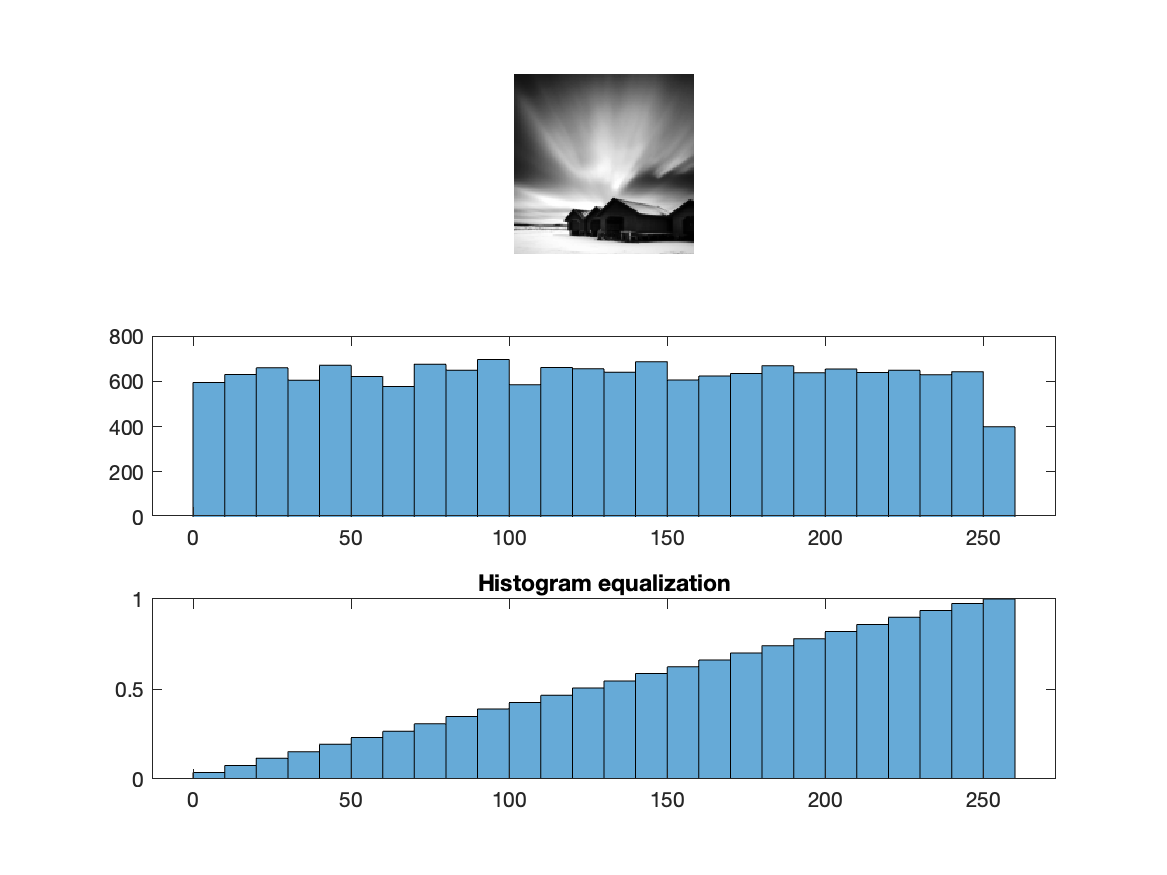
\includegraphics[width=120mm]{figures/Q16.png}
\caption{}
\label{fig:Q16}
\end{figure}

% Delete this section if you have no plot to submit.
% Change the size of the figure by changing the value in [width=300pt]

% Putting \autoref{fig:my_figure} in your text will refer to the corresponding figure label.
% Eg.: "\autoref{fig:my_figure} clearly shows that the large circle is larger than the small box."
% Read more about autoref here https://en.wikibooks.org/wiki/LaTeX/Labels_and_Cross-referencing#autoref

%\bibliographystyle{apalike}
%\bibliographystyle{abbrv}
%\bibliography{bibliography}

\end{document}